\documentclass{article}
\usepackage[utf8]{inputenc}
\usepackage[T2A]{fontenc}
\usepackage[russian]{babel}
\usepackage{graphicx}
\usepackage{amsmath}
\usepackage{amssymb}
\usepackage{bm}
\usepackage{mathtools}

\begin{document}
	
	\tableofcontents
	
	\newpage
	
	\section{NN}
	
	\textbf{Дано}
	
	$X \in \mathbb R ^{n \times p}$ --- множество объектов.
	
	$Y \in \mathbb{R}^n$ --- множество ответов.\\

	\textbf{Оптимизационная задача}
	$$Q(a, X^n) = \dfrac{1}{n} \sum\limits_{j=1}^n \mathcal{L} (a, x_i, y_i) \to \min_{\omega}.$$
	
	\textbf{Алгоритм (модель)}
	$$a(x, \omega) = \sigma \left( <\omega, x> \right) \sigma \left( \sum\limits_{j=1}^{p} \omega_j f_j(x) - \omega_0 \right),$$

	$\omega = (\omega_1, \ldots, \omega_p) \in \mathbb{R}^p$ --- вектор параметров.
	
	$\sigma: \mathbb{R} \to \mathbb{R}$ --- функция активации.
	
	$\omega_0$ --- порог активации.
	
	Если $\sigma(z) = sign(z)$, то $a(x, \omega)$ --- просто линейный классификатор. Уравнение $<\omega, x> = 0$ задает гиперплоскость, разделяющие классы в пространстве $\mathbb{R}^p$. Если вектор $x$ находится по одну сторону гиперплоскости с ее направляющим вектором $\omega$, то объект $x$ относится к классу $+1$, иначе к классу $-1$.\\
	
	\textbf{Задача регрессии}
	
	$\textbf{y} = \mathbb{R}.$
	
	$a(x_j, \omega) = \sigma(<\omega, x_j>).$

	$$Q(\omega; X^n) =  \sum\limits_{j=1}^{n} \mathcal{L} (<\omega, x_j>, y_j) = \sum\limits_{j=1}^{n} \left( \sigma (<\omega, x_j>) - y_j \right)^2 \to \min_{\omega}.$$
	
	При $\sigma(z) = z$ получаем многомерную линейную регрессию.\\
	
	\textbf{Задача классификации}
	
	$\textbf{y} = \{-1, 1\}.$
	
	$a(x_j, \omega) = sign <\omega, x_j>.$
	
	$$Q(\omega; X^n) =  \sum\limits_{j=1}^{n} \mathcal{L} (<\omega, x_j>, y_j) = \sum\limits_{j=1}^{n} \left[ y_j <\omega, x_j> < 0 \right]^2 \to \min_{\omega}.$$
	
	\textbf{Функции активации}
	\begin{itemize}
		\item логистическая (сигмоидная) функция: $\sigma(z) = \dfrac{1}{1+e^{-az}}, a \in \mathbb{R}$;
		\item гиперболический тангенс: $\sigma(z) = \dfrac{e^{az} - e^{-az}}{e^{az} + e^{-az}}, a \in \mathbb{R}$;
		\item softmax: $SM_i(z) = \dfrac{e^{z_i}}{\sum\limits_{k=1}^{K} e^{z_k}}$;
		\item выпрямитель: $ReLU(p) = \max(0, p)$.
	\end{itemize}
	
	\textbf{Функции потерь}
	\begin{itemize}
		\item MSE
		\item CE (кросс энтропия)
		\item BCE (бинарная кросс-энтропия)
	\end{itemize}
	
	\textbf{Расчет весов}
	
	Backpropagation (метод обратного распространения ошибки), стохастический градиентный спуск.\\
	
	\textbf{Выбор гиперпараметров}
	\begin{itemize}
		\item число слоев
		\item число нейронов
		\item число связей для каждого нейрона
		\item и т.д. (число эпох, batch size)
		\item динамическое добавление нейронов
		\item удаление избыточных связей (OBD)
	\end{itemize}

	\newpage

	\section{CNN}

	\subsection{Особенности построения нейронных сетей для изображений (Convolutional Neural Networks)}
	
	\begin{itemize}
		\item локальная скореллированность пикселей
		\item распределенность признака
		\item возможность трансформации шаблонов (поворот, смещение, масштабирование)
	\end{itemize}

	Входной сигнал изображения подается на вход нейрона только в пределах ограниченной области, как правило, квадратной, например, 3х3 пикселей. Затем, эта область смещается вправо на заданный шаг, допустим, 1 пиксель и входы подаются уже на второй нейрон. Так происходит сканирование всего изображения. Причем, весовые коэффициенты для всех нейронов этой группы – одинаковые.

	После этого сканирование изображения повторяется, но с другим набором весовых коэффициентов. Получаем вторую группу нейронов. Затем, третью, четвертую и в общем случае имеем n различных групп. Так формируется первый скрытый слой нейронов сверточной НС.\\
	
	\noindent 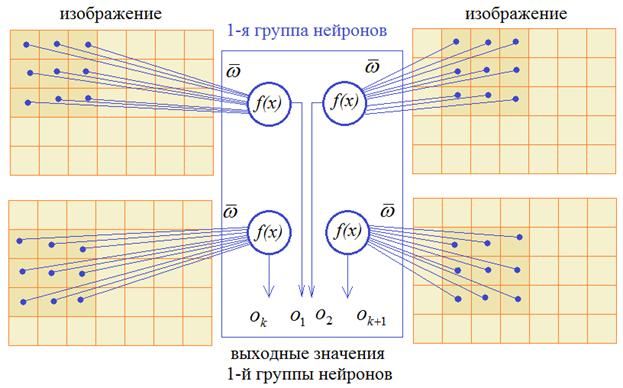
\includegraphics[width=\textwidth]{pic1.jpg}
	\begin{center}
		Рис. входной сигнал
	\end{center}

	\subsection{Свертка}
	
	Свёртка, конволюция — операция в функциональном анализе, которая при применении к двум функциям 
	$\displaystyle f$
	и 
	$\displaystyle g$
	возвращает третью функцию, соответствующую взаимнокорреляционной функции 
	$\displaystyle f(x)$
	и 
	$\displaystyle g(-x)$
	. Операцию свёртки можно интерпретировать как «схожесть» одной функции с отражённой и сдвинутой копией другой. Понятие свёртки обобщается для функций, определённых на произвольных измеримых пространствах, и может рассматриваться как особый вид интегрального преобразования. В дискретном случае свёртка соответствует сумме значений 
	$\displaystyle f$
	с коэффициентами, соответствующими смещённым значениям 
	$\displaystyle g$
	, то есть 
	$$\displaystyle (f*g)(x)=f(1)g(x-1)+f(2)g(x-2)+f(3)g(x-3)+\dots$$
	
	\textbf{Определение свертки}
	
	Пусть 
	$\displaystyle f,g:\mathbb {R} ^{n}\to \mathbb {R}$
	— две функции, интегрируемые относительно меры Лебега на пространстве 
	$\displaystyle \mathbb {R} ^{n}$
	. Тогда их свёрткой называется функция 
	$\displaystyle f*g:\mathbb {R} ^{n}\to \mathbb {R}$
	, определённая формулой
	
	$$\displaystyle (f*g)(x) \displaystyle {\stackrel {\mathrm {def} }{=}}\ \int \limits _{\mathbb {R} ^{n}}f(y)\,g(x-y)\,dy=\int \limits _{\mathbb {R} ^{n}}f(x-y)\,g(y)\,dy.$$
	
	\subsection{Карта признаков (feature map / activation map)}
	
	Пусть на вход нейросети подается изображение размером $M \times N$. Обозначим его как отображение $x: Z \times Z \to \mathbb{R}^3$. Введем ядро свертки, представляющее собой набор весов $W: Z \times Z \to \mathbb{R}^3$. Рассмотрим следующее отображение:
	$$f(i,j): Z \times Z \to \mathbb{R};$$
	$$f(i,j) = \sigma((W \cdot x)(i,j) + b);$$
	где $b$ --- смещение, $\sigma$ --- нелинейная функция. Вектор из таких отображений, построенный на разных ядрах $W_k$ и смещениях $b_k$ называется \textbf{feature map}.\\
	
	\subsection{Ядро фильтра}
	
	Ядро фильтра --- набор коэффициентов $\omega$ размера, например, $3 \times 3$.\\
	$$ W = \begin{matrix}
		\omega_{11} & \omega_{12} & \omega_{13}\\
		\omega_{21} & \omega_{22} & \omega_{23}\\
		\omega_{31} & \omega_{32} & \omega_{33}
	\end{matrix}$$
	Мы имеем $3 \cdot 3 + 1 = 10$ настраиваемых параметров.

	Матрица данных (изображение)
	$$
	\begin{matrix}
		x_{11} & x_{12} & x_{13} & x_{14} & x_{15}\\
		x_{21} & x_{22} & x_{23} & x_{24} & x_{25}\\
		x_{31} & x_{32} & x_{33} & x_{34} & x_{35}\\
		x_{41} & x_{42} & x_{43} & x_{44} & x_{45}\\
		x_{51} & x_{52} & x_{53} & x_{54} & x_{55}\\
	\end{matrix}
	$$
	
	Свертка общая формула\\
	$v_{k,m} = \sum\limits_{i=1}^{3} \sum\limits_{j=1}^{3} x_{i+k, j+m} \cdot \omega_{ij} + \omega_0, \; k,m = 0, \dots, n$
	
	Свертка пример\\
	$v_{0,0} = \sum\limits_{i=1}^{3} \sum\limits_{j=1}^{3} x_{i,j} \cdot \omega_{ij} + \omega_0$\\
	$v_{0,1} = \sum\limits_{i=1}^{3} \sum\limits_{j=1}^{3} x_{i,j+1} \cdot \omega_{ij} + \omega_0$
	
	Берем часть изображения. Если сумма произведений значения каждого пикселя на весовой коэффициент превышает некоторое пороговое значение, это значит что мы выявили паттерн, функция активации срабатывает и сигнал передается на следующий слой.\\
	
	\subsection{Пример паттерна}
	
	Пусть у нас есть фильтр, способный определять вертикальную линию, где 0 --- белый цвет, 1 --- черный цвет (либо наоборот).
	$$W = \begin{matrix}
		0 & 1 & 0\\
		0 & 1 & 0\\
		0 & 1 & 0
	\end{matrix}$$
	Тогда если у нас будет следующее изображение
	$$x = \begin{matrix}
		0 & 1 & 0\\
		0 & 1 & 0\\
		0 & 1 & 0
	\end{matrix}$$
	то
	$v_{0,0} = 1 \cdot 1 + 1 \cdot 1 + 1 \cdot 1$\\
	Если же у нас будет длинная вертикальная линия
		$$x = \begin{matrix}
		0 & 1 & 0\\
		0 & 1 & 0\\
		0 & 1 & 0\\
		\vdots & \vdots & \vdots\\
		0 & 1 & 0
	\end{matrix}$$
	то наши коэффициенты при каждом сдвиге будут следующими
	\begin{align*}
		v_{0,0} = 1 \cdot 1 + 1 \cdot 1 + 1 \cdot 1\\
		v_{1,0} = 1 \cdot 1 + 1 \cdot 1 + 1 \cdot 1\\
		\vdots\\
		v_{n,0} = 1 \cdot 1 + 1 \cdot 1 + 1 \cdot 1
	\end{align*}
	На каждом шаге мы будем получать большие коэффициентые и сигнал будет переходить на следующих слой. Т.е. фильтр позволяет выделять характерные участки на изображении в соответствии с конфигурацией весовых коэффициентов.
	
	Благодаря такому подходу нейроны каждой группы активируются тогда, когда на участке изображения появляется фрагмент, подходящий под их ядра.
	
	\subsection{Пример изображения}
	
	Давайте представим, что у нас имеется схематичное изображение дома и мы пропустим его через вот такие ядра:\\
	
	\noindent 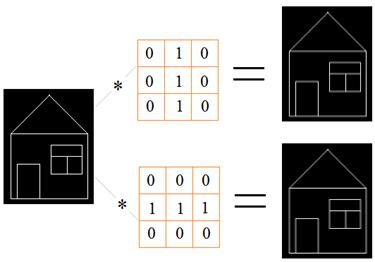
\includegraphics[width=\textwidth]{pic4.jpg}
	\begin{center}
		Рис. пример
	\end{center}
	
	На выходе получаем отчетливые вертикальные линии в первом случае и горизонтальные – во втором случае. Все остальные линии стали более бледными. То есть, фильтр позволяет выделять характерные участки на изображении в соответствии с конфигурацией весовых коэффициентов. Благодаря такому подходу, нейроны каждой группы активизируются, когда на участке изображения появляется фрагмент, подходящий под их ядра:\\
	
	\noindent 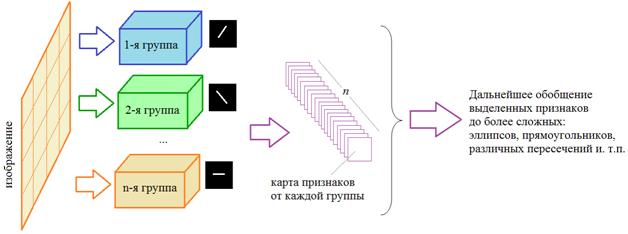
\includegraphics[width=\textwidth]{pic5.jpg}
	\begin{center}
		Рис. каналы
	\end{center}

	И на выходе формируется набор карт признаков, которые называются каналами. Значимые величины в каждой карте показывают наличие признака в строго определенном месте изображения. Если таких признаков будет несколько (на разных участках изображения), то на выходе будут активироваться несколько нейронов, связанных с этими областями. Благодаря этому, следующие слои сверток могут обобщать найденные особенности до более сложных, например, эллипсов, прямоугольников, различных пересечений линий и т.п.

	Разумеется, значения карт признаков – это выходы функций активации нейронов, то есть, здесь, все как обычно: сумма (свертка) проходит через функцию активации и формируются выходные значения:

	$v_{k,m} = \sum\limits_{i=1}^{3} \sum\limits_{j=1}^{3} x_{i+k, j+m} \cdot \omega_{ij} + \omega_0, \; k,m = 0, \dots, n$\\
	
	\subsection{Полноцветное изображение}
	
	\begin{figure}[h]
		\begin{minipage}[h]{0.49\linewidth}
			\center{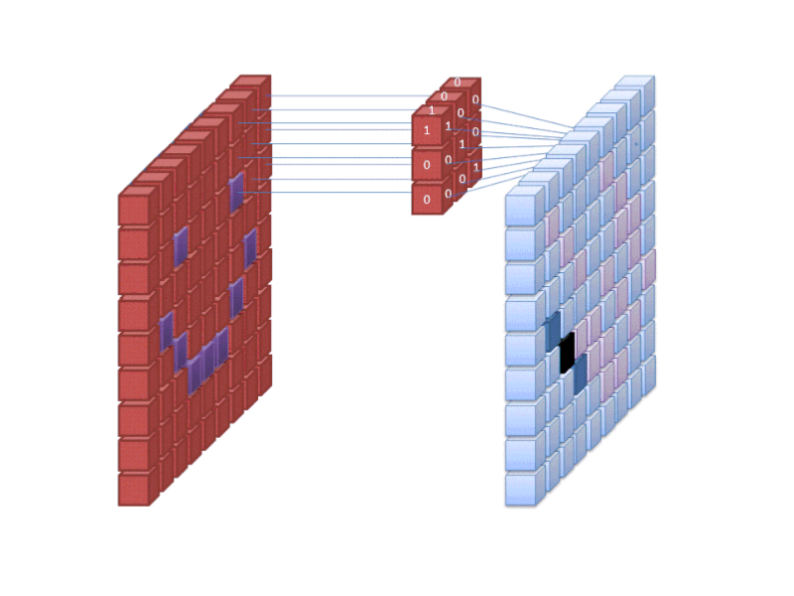
\includegraphics[width=0.7\linewidth]{pic13.jpg} \\ Рис. одноцветное}
		\end{minipage}
		\hfill
		\begin{minipage}[h]{0.49\linewidth}
			\center{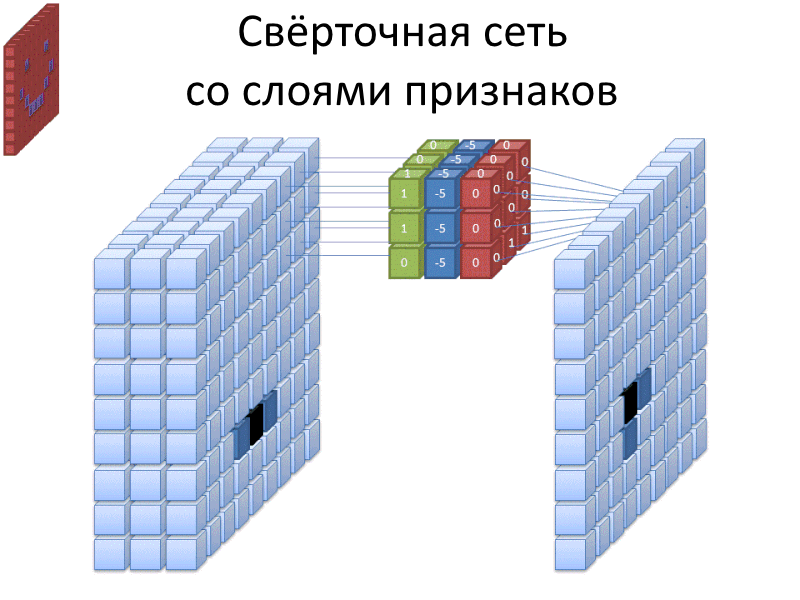
\includegraphics[width=0.7\linewidth]{pic14.jpg} \\ Рис. полноцветное}
		\end{minipage}
	\end{figure}
	
	Но мы рассмотрели простейший вариант, когда на вход подавалось одноканальное изображение, например, в градациях серого. Если обрабатывается полноцветное изображение, представленное, например, тремя цветовыми компонентами RGB, то каждая цветовая компонента сначала преобразовывается своим отдельным, независимым ядром, затем, вычисленные карты признаков, складываются, к ним добавляется смещение и формируется единая итоговая матрица признаков, которая проходит через функцию активации нейронов и получаются выходные значения на соответствующем канале.\\
	
	\noindent 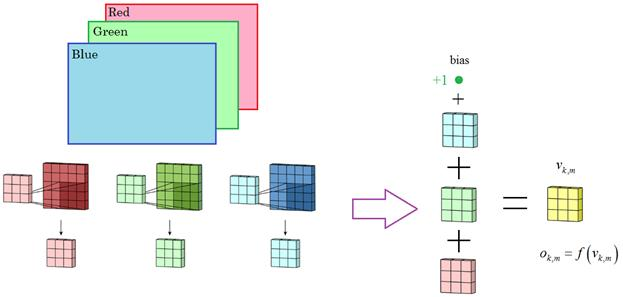
\includegraphics[width=\textwidth]{pic6.jpg}
	\begin{center}
		Рис. полноцветное изображение
	\end{center}
	
	\subsection{Функции активации}
	
	После того, как карта признаков изображения была создана, значения, представляющие изображение, передаются через функцию активации или слой активации, например
	\begin{itemize}
		\item ReLU
	\end{itemize}

	\subsection{MaxPooling}

	Далее размерность карт сокращается
	\begin{itemize}
		\item MaxPooling – отбор наибольших значений;
		\item MinPooling – отбор наименьших значений;
		\item AveragePooling – отбор средних значений.
	\end{itemize}

	Давайте представим, что мы хотим вдвое уменьшить линейные размеры карты признаков. В этом случае ее можно покрыть непересекающимися блоками 2х2 пиксела и в каждом блоке оставить только максимальные значения:
	
	\noindent 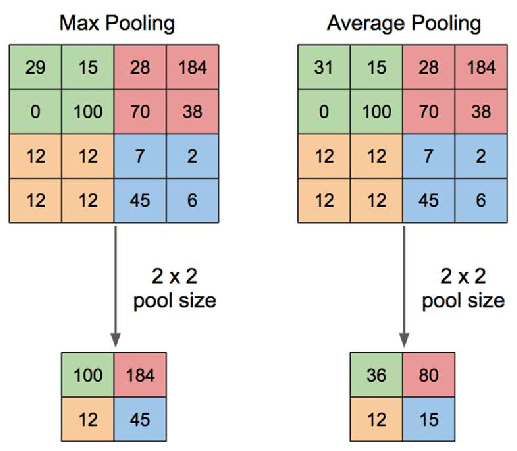
\includegraphics[width=\textwidth]{pic15.png}
	\begin{center}
		Рис. maxpooling \& averagepooling
	\end{center}

	\noindent 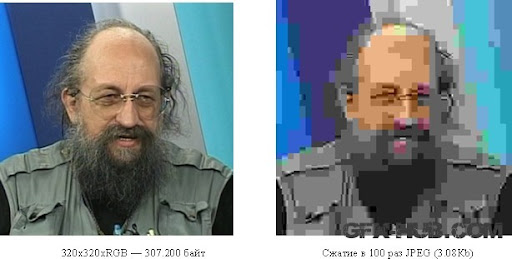
\includegraphics[width=\textwidth]{pic16.jpg}
	\begin{center}
		Рис. cжатие в 100 раз
	\end{center}

	\subsection{Итоговая архитекрутра}
	
	Финальная архитектура будет выглядеть следующим образом: на вход подается изображение 32 на 32 пикселя. В первом слое мы получаем набор из 10 карт признаков и сжимаем их при помощи MaxPooling. Далее те же операции повторяются во втором скрытом слое. Число слоев можно увеличивать и далее. В конце вычисленные карты признаков подаются на вход обычной полносвязной NN. Конечный этап сверточной NN в задачах классификации, обычно, завершается полносвязной NN, на выходе которой получаем вероятности принадлежности к тому или иному классу.

	\noindent 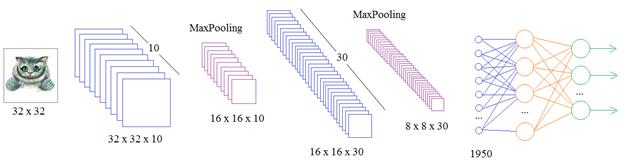
\includegraphics[width=\textwidth]{pic12.jpg}
	\begin{center}
	Рис. итоговая архитектура
	\end{center}
\end{document}
